% !TeX root = RJwrapper.tex
\title{Opening Up Official Statistics in R with \pkg{pxweb}}
\author{by M\r{a}ns Magnusson and Leo Lahti}

\maketitle

\abstract{
The pxweb package provides an interface from R to statistical databases published through the PxWeb API.
PxWeb is used by national, regional, and international statistical organizations to disseminate official statistics in multidimensional tables.
The package supports discovery of API resources, construction and validation of queries, retrieval and parsing of data and metadata, conversion to standard R data structures, extraction of comments, and citation of retrieved data.
This article introduces the motivation and design of the pxweb R package, show the use of both PxWeb API version 1 and version 2, and provides a reproducible case study using official statistics.
}

% Keywords: open data, citing data, public data, pxweb, PC-Axis, R

\section{Introduction}

Open data science workflows rely heavily on algorithmic tools for data retrieval.
Automating data discovery, retrieval, integration, and citation gives users more time for analysis and interpretation.
It also supports reproducible research \citep{Gandrud13, Boettiger2015} by making data acquisition explicit and repeatable.

Official statistics are a particularly important type of public data \citep{UNGA_2014_FPOS}.
National statistical institutes (NSI) and international agencies publish large amounts of data in a vast number of areas, such as demography, economics, health, infrastructure, climate, to name a few \citep{UNGA_2014_FPOS,WorldBank_WDI}.
Such data are often multidimensional, geographically detailed, and updated over long time periods.
During the last decade such data has become increasingly available through open web-based application programming interfaces (API).
Opening statistical resources through public web APIs is, however, only the first step to enable use of statistical data.
Users also need software that can bridge the gap between online statistical databases and analysis in statistical programming environments such as R.

There are many dedicated software packages that simplify and automate analysis workflows.
They take into account variations in raw data formats, access details, metadata conventions, and typical use cases so that users can avoid repetitive programming tasks and reduce the risk of processing errors \citep{GrovesLyberg2010}.
In R, several packages support programmatic data retrieval in different ways, from specific sources \citep{Lahti17eurostat, WDI}, broader compiled sources such as economic and financial time-series data \citep{pdfetch}, generic data sources \citep{szocs2020webchem, caro2017intsvy}, or specific statistical standards, such as the SDMX data standard \citep{rsdmx}.

The \CRANpkg{pxweb} package \citep{pxweb} fills a complementary role: it provides a general R interface to databases exposed through the PxWeb application programming interface (API) \citep{PxToolsPxWeb2Intro}.
The package can navigate PxWeb resources, fetch metadata, construct and validate queries, retrieve data, and convert responses into standard R data structures.
The package includes 46 API catalogue entries and supports versions 1 and 2 of the PxWeb API \citep{PxToolsPxWeb2Intro}.

Data citation is another motivation for the package.
Data reuse should document source organizations, accessed resources, version information, and retrieval times where possible \citep{Parsons2019}.
The \CRANpkg{pxweb} package helps standardize and streamline this process for PxWeb data by collecting source information from the API and data objects and by encouraging users to cite both the retrieved data and the software used to retrieve them for full reproducibility.

The \CRANpkg{pxweb} package was first released on CRAN in 2014 and was substantially upgraded in 2018 and 2026.
Recent development in 2026 has added support for the PxWeb API version 2, including table search, \texttt{JSON-stat2} responses, v2 metadata, codelists, value sets, aggregation helpers, and observation status comments.
Here we introduce the use of \citep{pxweb} version 1.0.0. \footnote{The package is now version 0.19.2 at CRAN. Version 1.0.0 will be released on CRAN to accompany publication of this article. Then also this footnote will be removed.}
The current package is part of the rOpenGov open data science project \citep{Lahti13icml}.

\subsection[PxWeb and PC-Axis]{PxWeb and PC-Axis}
\label{sec:pxweb-pcaxis}

PxWeb is a web application and API for disseminating PC-Axis-type statistical data \citep{PxToolsPxWeb2Intro}.
PC-Axis data are data files typically organized as multidimensional tables with dimensions such as region, time, sex, age, indicator, or content.
The PX software family (including both PC-Axis and PxWeb) is used by a large number of NSIs, e.g. Statistics Sweden, Statistics Finland, and Statistics Norway to name a few \citep{SCBPxPrograms,StatisticsFinlandPxSuite,StatisticsNorwayAPI}.
PxWeb exposes data and metadata through hypertext transfer protocol (HTTP) endpoints that can be accessed programmatically.

The PX file format stores metadata and data in a single file.
% The specification lists 1990 as the introduction year for \code{CONTENTS}, \code{DATA}, \code{MATRIX}, \code{STUB}, and \code{CODES} \citep[Section~3.1]{SCBPxFileFormat2013}.
Statistics Sweden describes PX as a standard format for statistics files used by many statistical offices and as the basis for tools such as PxWin, PxWeb, and PxEdit \citep{SCBPxPrograms}.
PxWeb extends this file-oriented tradition to online dissemination by publishing statistical tables through web interfaces \citep{PxToolsPxWeb2Intro}.

Recently, PxWeb API version 2 emerged as a joint Statistics Sweden and Statistics Norway project initiated in January 2024 because the older PxWeb version 1 interface had become difficult to develop further and user needs were changing.
Public test versions appeared in 2024, followed by a PxWebApi v2 release in September 2025 and a PxWeb 2 release in October 2025.
The new API modernizes the infrastructure through GET URL support, JSON-stat2 output, improved filtering, language handling, and richer metadata access \citep{PxToolsPxWeb2Process,PxToolsPxWeb2Plans,PxToolsPxWebApi2UserGuide}.

From the perspective of an R user, PxWeb APIs have three important parts.
First, a table query must be constructed from table metadata.
Second, the data response has to be retrieved and converted into an analysis-ready format in R.
Third, the downloaded data should be easy to cite to facilitate provenance and reproducibility.
The \CRANpkg{pxweb} package handles all three parts for the R user.

The \CRANpkg{pxweb} package is solely designed for PxWeb APIs, while packages such as \CRANpkg{pxR} focus on parsing PC-Axis files \citep{pxR}.
This distinction is important because API access requires metadata discovery, query construction, request validation, and response parsing rather than only local file import.

Since PxWeb installations are configured by individual providers, such as NSIs, API version support and request limits are server-level properties rather than package-level constants.
The \CRANpkg{pxweb} package therefore collects available configuration metadata, including version 1 and 2 \code{config} responses, and uses this information when validating requests, making calls, and splitting large downloads.

\subsection{Related software}
\label{sec:related}

The R ecosystem contains several packages for accessing official statistics and other public data.
However, these tools differ in the publication systems and data models they work with.
Table~\ref{tab:related-software} summarizes the main distinctions.
Provider-specific packages, such as \CRANpkg{eurostat} \citep{Lahti17eurostat} and \CRANpkg{WDI} \citep{WDI}, provide convenient access to individual statistical sources.
Broader data-retrieval packages, such as \CRANpkg{pdfetch} \citep{pdfetch}, \CRANpkg{webchem} \citep{szocs2020webchem}, and \CRANpkg{intsvy} \citep{caro2017intsvy}, support data collection in specific areas, such as finance, chemistry, and education.
The \CRANpkg{rsdmx} package supports the Statistical Data and Metadata eXchange (SDMX) standard, which is an important alternative standard for statistical data exchange \citep{rsdmx,willekens2023sdmx}.
In Python, pxwebpy provides access to PxWeb API version 2 \citep{pxwebpy}.

In this landscape, \CRANpkg{pxweb} focus on PxWeb APIs.
It provides a common interface for (1) discovering databases and tables, (2) inspecting metadata, (3) constructing valid queries, (4) respecting server limits, (5) retrieving data, and (6) retaining comments and citation information across statistical organisations that publish through PxWeb APIs.
This makes \CRANpkg{pxweb} complementary to existing tools.
The contribution of \CRANpkg{pxweb} is to support the common case where official statistics are distributed through PxWeb APIs and where users need a general, metadata-aware, and reproducible interface from R.

\begin{table}[!htbp]
\centering
\small
\begin{tabular}{>{\raggedright\arraybackslash}p{0.25\textwidth}>{\raggedright\arraybackslash}p{0.22\textwidth}>{\raggedright\arraybackslash}p{0.43\textwidth}}
\toprule
Software type & Packages & Relation to \CRANpkg{pxweb}\\
\midrule
Provider-specific data clients &
\CRANpkg{eurostat}, \CRANpkg{WDI} &
Focus on one data provider or data family \\
Generic data retrieval tools &
\CRANpkg{pdfetch}, \CRANpkg{webchem}, \CRANpkg{intsvy} &
Retrieve broad data sources but do not target PxWeb APIs\\
PX/PC-Axis file tools &
\CRANpkg{pxR} &
Work with local \code{.px} files\\
SDMX clients &
\CRANpkg{rsdmx} &
Access data via the alternative SDMX standard.\\
Python PxWeb API client &
pxwebpy &
Accesses PxWeb API version 2 from Python\\
Downstream domain packages &
\CRANpkg{geofi} \citep{geofi} &
Specialized workflows on top of official-data access\\
\bottomrule
\end{tabular}
\caption{\label{tab:related-software}Related software to \CRANpkg{pxweb}.}
\end{table}

\section[The pxweb package]{The \CRANpkg{pxweb} package}
\label{sec:package-design}

The \CRANpkg{pxweb} package is designed for R users who need to retrieve official statistics reproducibly from R without writing specific HTTP requests.
Its core design goal is to provide a stable R workflow across PxWeb APIs while preserving metadata where it affects query construction, codelists, comments, and citation.
The package is licensed under the BSD-2-Clause (aka FreeBSD) license, consistent with common practice for research software \citep{Morin2012}.

Version 1.0.0 described here exports 39 functions, but the main workflow uses a smaller set of recommended functions.
The central workflow is built around the \code{pxweb\_get()} function, which retrieves hierarchy levels, table metadata, or table data depending on the supplied PxWeb version, URL and query.
The helper \code{pxweb\_get\_data()} wraps the same workflow and returns a \code{data.frame}.
Additional methods, such as \code{as.data.frame()}, integrate the outputs directly with \CRANpkg{tidyverse} workflows \citep{tidyverse2019}, allowing users to move from data retrieval to tidy data analysis \citep{Wickham2014tidy}.
Query construction is handled by \code{pxweb\_query()} together with query construction helper functions \code{pxweb\_all()}, \code{pxweb\_latest()}, and \code{pxweb\_aggregation()}.
Table~\ref{tab:workflow-functions} summarises the main user-facing functions and methods by their role in the recommended workflow.

\begin{table}[!htbp]
\centering
\small
\begin{tabular}{>{\raggedright\arraybackslash}p{0.24\textwidth}>{\raggedright\arraybackslash}p{0.68\textwidth}}
\toprule
Workflow part & Recommended functions and methods\\
\midrule
Search and discovery &
\begin{minipage}[t]{0.68\textwidth}\raggedright
\code{pxweb\_search()}, \code{pxweb\_interactive()},
\code{pxweb\_api\_catalogue()}\end{minipage}\\
Metadata &
\begin{minipage}[t]{0.68\textwidth}\raggedright
\code{pxweb\_get()}, \code{pxweb\_codelists()}\end{minipage}\\
Query &
\begin{minipage}[t]{0.68\textwidth}\raggedright
\code{pxweb\_query()}, \code{pxweb\_validate\_query\_with\_metadata()},
\code{pxweb\_all()}, \code{pxweb\_latest()},
\code{pxweb\_aggregation()}, \code{pxweb\_valueset()}\end{minipage}\\
Retrieval &
\begin{minipage}[t]{0.68\textwidth}\raggedright
\code{pxweb\_get()}, \code{pxweb\_get\_data()}\end{minipage}\\
Conversion &
\begin{minipage}[t]{0.68\textwidth}\raggedright
\code{as.data.frame()}\end{minipage}\\
Comments and citation &
\begin{minipage}[t]{0.68\textwidth}\raggedright
\code{pxweb\_data\_comments()}, \code{pxweb\_cite()}\end{minipage}\\
\bottomrule
\end{tabular}
\caption{\label{tab:workflow-functions}Recommended \CRANpkg{pxweb}
functions and methods.}
\end{table}

Internally, the package represents API URLs, metadata, data, comments, and query objects with S3 classes.
This allows common operations to behave consistently across API versions.
The package uses \CRANpkg{httr} for HTTP requests and \CRANpkg{jsonlite} for JSON parsing \citep{httr,jsonlite}.
Table~\ref{tab:object-classes} summarizes the main object classes used in ordinary workflows.

\begin{table}[!htbp]
\centering
\small
\begin{tabular}{>{\raggedright\arraybackslash}p{0.25\textwidth}>{\raggedright\arraybackslash}p{0.65\textwidth}}
\toprule
Class & Role and common methods\\
\midrule
\code{pxweb} &
Represents an API endpoint created from a URL; printed with \code{print()}\\
\code{pxweb\_metadata} &
Stores table metadata and selected version 2 metadata; inspected with \code{as.data.frame()} and \code{pxweb\_codelists()}, and used by \code{pxweb\_validate\_query\_with\_metadata()}\\
\code{pxweb\_query} &
Represents selections to send to the API; created with \code{pxweb\_query()} and converted to JSON with \code{pxweb\_query\_as\_json()}. For simple selections, \code{pxweb\_query\_as\_rcode()} prints an R list of value codes; it does not preserve codelist selections.\\
\code{pxweb\_data}, \code{pxweb\_data\_v2} &
Represent retrieved table data for API versions 1 and 2; created by \code{pxweb\_get()}, converted with \code{as.data.frame()} or \code{as.matrix()}, and cited with \code{pxweb\_cite()}\\
\code{pxweb\_data\_comments} &
Collects dataset, dimension, value, and observation comments from \code{pxweb\_data\_comments()}; printed or converted to a \code{data.frame} for inspection and reporting\\
\bottomrule
\end{tabular}
\caption{\label{tab:object-classes}Main S3 object classes used by
\CRANpkg{pxweb} in ordinary data-access workflows.}
\end{table}

The API catalogue is a practical layer on top of the API functionality.
It stores provider URL templates, available languages, version paths, aliases, and citation metadata.
Users can rely on the catalogue for common APIs or pass explicit PxWeb URLs for APIs that are not already part of the package.
The current catalogue contains 46 entries covering national, regional, and international statistical resources.
The complete list is given in the appendix (Table~\ref{tab:api-catalogue}).
% Since PxWeb installations are maintained by the individual data providers, the catalogue is a tested convenience layer rather than a guarantee that every provider will remain permanently available.
% Hence, users can pass explicit PxWeb URLs when catalogue entries change or are missing.
At the time of writing, the catalogue entries point mainly to version 1 API paths.
Version 2 APIs can also be used by passing explicit PxWeb URLs.

A central implementation detail is that user-supplied URLs are first converted into a \code{pxweb} object.
The constructor (1) parses the URL, (2) detects whether the endpoint belongs to PxWeb API version 1 or 2, (3) retrieves provider configuration metadata, and (4) stores call history in a temporary cache.
Provider configuration is normalised into a common internal representation with the number of calls allowed per time window, the length of that time window, and the maximum number of downloadable values or cells.
This lets the same retrieval workflow use version 1 \code{?config} responses and version 2 \code{/config} responses through the same interface.

Support for PxWeb API version 2 is expressed in the same workflow as version 1.
Version 2 tables use separate metadata and data URL endpoints and return JSON-stat2 by default \citep{PxToolsPxWeb2Intro}.
The \CRANpkg{pxweb} package (1) detects v2 URLs, (2) builds the corresponding data URL, (3) constructs the v2 query body, and (4) adds query parameters for codelists and output values when needed.
This keeps the user workflow similar across API versions, even though the underlying URL and request details differ.

For data requests, \code{pxweb\_get()} first fetch table metadata, then adds mandatory variables (if needed), validates the query against the metadata, and computes any required download batches before making data requests.
Version 1 tables are queried with the table URL and a JSON request body, whereas version 2 tables use the corresponding \code{/tables/\{id\}/data} URL with version-specific query parameters.
The returned data objects are parsed into package-specific S3 objects.

Large queries of statistical tables can exceed server-side limits.
This makes it hard for individual user.
They need to download the data in multiple batches by partitioning the original query in smaller pieces, download each query, and then combine them into one dataset.
The \code{pxweb} package handles this automatically when the query can be split within the provider's limit.
This procedure can be viewed as a greedy multidimensional query-partitioning heuristic.
Given the provider's maximum downloadable size, the algorithm first identifies splittable dimensions from the table metadata.
Time variables can be split, and so can variables marked as eliminable in the provider metadata, meaning that the API allows them to be omitted or partitioned.
Content variables and top or bottom selections are kept intact because they affect the meaning or ordering of the returned values.
The partitioning procedure then evaluates candidate orderings of the splittable dimensions and, for each ordering, greedily chooses the largest dimension chunks that keep each subquery below the provider limit.
The ordering with the smallest resulting number of batches is then used to download the query.
For the typical case of fewer than seven splittable dimensions, all orderings are evaluated.
Otherwise, a random sample of orderings is used to keep computation bounded.

% For requests that return parsed data, the package retrieves batches sequentially and holds them in memory until it combines them.
% Batching works within the provider's per-response limit, but both the batches and the combined result must fit in memory.

The \code{pxweb} package follows common software engineering practices, including version control, automated tests, API fixtures, continuous integration, and test workflows for selected APIs \citep{PerezRiverol2016}.
The default local test suite uses mocked and offline-safe tests, and live tests run in continuous integration (CI) on GitHub.



\subsection{Functionality}
\label{sec:functionality}

The package supports the full workflow shown in Figure~\ref{fig:workflow-model}: search and discovery, metadata inspection, query construction, retrieval, conversion, comments, and citation.

\begin{figure}[t!]
\centering
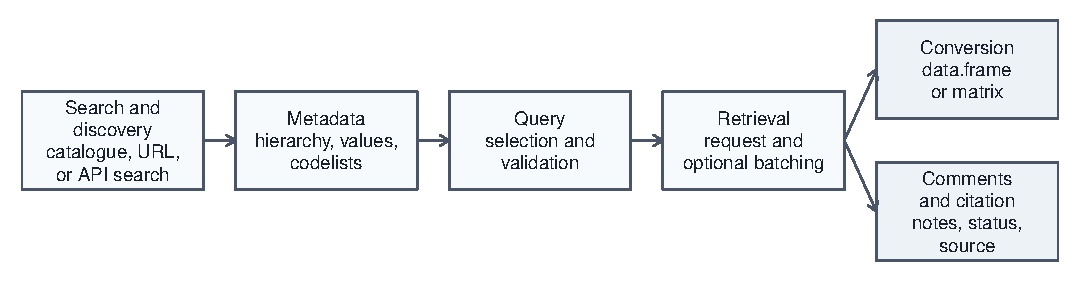
\includegraphics[width=\textwidth]{figs/workflow-model}
\caption{\label{fig:workflow-model}Main \CRANpkg{pxweb} workflow.
After retrieval, the same data object can be converted for analysis or used to extract comments and generate a citation (or both).}
\end{figure}

For released versions, installation from CRAN follows the standard procedure in R.

\begin{example}
install.packages("pxweb")
library("pxweb")
\end{example}

Search and discovery start either from the bundled API catalogue, for PxWeb API version 1, from an explicit URL, or, for PxWeb API version 2, from table search.
The following example searches Statistics Sweden's PxWeb API version 2 for a population table.

\begin{example}
search_results <- pxweb_search(
  query = "population marital status",
  api_url = "https://statistikdatabasen.scb.se/api/v2",
  lang = "en",
  page_size = 5
)

print(search_results[, c("id", "label")], row.names = FALSE, right = FALSE)
\end{example}

\begin{example}
 id      label
 TAB638  Population by region, marital status, age and sex.  Year 1968-2024
 TAB5557 Population by region, marital status, age and sex. Year 2025
 TAB2819 Mean population by region, marital status, age and sex. Year 2006-2024
 TAB6759 Mean population by region, marital status, age and sex.  Year 2025
 TAB6570 Population per region by marital status and sex. Year 2010-2025
\end{example}

The results include population tables for 1968--2024 and for 2025.
We select \code{TAB638} for the longer period by matching its ID, rather than relying on the order of the results, and extract the table metadata URL.

\begin{example}
url <- search_results$metadata_url[search_results$id == "TAB638"]
\end{example}

Metadata are retrieved with \code{pxweb\_get()} when no query is supplied.
The returned metadata object describes the table dimensions, values, labels, and version-specific metadata needed for query validation and data retrieval.
Version 2 APIs may also expose aggregation codelists and value sets, which can be inspected with \code{pxweb\_codelists()}.

\begin{example}
meta <- pxweb_get(url)
age_codelists <- pxweb_codelists(meta, variable = "Alder")
age_codelists[, c("id", "type", "label")]
\end{example}

\begin{example}
              id        type                          label
1 agg_Ålder10årJ Aggregation             ´10-year intervals
2   agg_Ålder5år Aggregation               5-year intervals
3   vs_Ålder1årA    Valueset        Age, 1 year age classes
4   vs_ÅlderTotA    Valueset Age, total, all presented ages
\end{example}

In this example the English metadata endpoint returns English labels, while the \code{id} values remain identifiers that are passed unchanged to query helper functions.
The five-year age aggregation can therefore be selected from the metadata and stored as an object before query construction.

Queries can be written as named R lists and converted to \code{pxweb\_query} objects when needed.
For codelists, the returned \code{id} column is passed to aggregation or value-set helpers.
Query helper functions express common selection patterns such as "all values", "the latest time period", top or bottom selections, aggregations, and value sets.
Queries are validated against the metadata of the table before calling the PxWeb API.

\begin{example}
age_5_year_id <- age_codelists$id[age_codelists$label == "5-year intervals"]

query <- list(
  Region = "00",
  Civilstand = "OG",
  Alder = pxweb_aggregation(age_5_year_id),
  Kon = c("1", "2"),
  ContentsCode = "BE0101N1",
  Tid = pxweb_latest()
)

px_query <- pxweb_query(query)
\end{example}

Retrieval is handled by \code{pxweb\_get()}.
Users who want a \code{data.frame} directly can instead use
\code{pxweb\_get\_data()}.
The same workflow handles version 1 and version 2 URLs, constructs the appropriate request body, and splits large supported queries into batches when needed.

\begin{example}
px_data <- pxweb_get(url, query = query)
\end{example}

Conversion methods turn PxWeb responses into standard R objects.
Users can choose whether column names and variable values use provider \code{label} or \code{code}.

\begin{example}
px_df <- as.data.frame(
  px_data,
  column.name.type = "code",
  variable.value.type = "code"
)
\end{example}

Finally, PxWeb responses may include comments, notes, or status information.
The \CRANpkg{pxweb} package enable access to these through \code{pxweb\_data\_comments()}, with support for both version 1 comments and version 2 dataset notes, dimension notes, value notes, and observation status comments.
Citation support is provided by \code{pxweb\_cite()}, which prints citation information for the retrieved data source and the \CRANpkg{pxweb} package itself.

\begin{example}
comments <- pxweb_data_comments(px_data)
pxweb_cite(px_data)
\end{example}

\section{Case study}
\label{sec:case-study}

We illustrate the package with a Statistics Sweden population table that is both familiar official statistics and technically useful for showing large queries.
The example uses Statistics Sweden's PxWeb API version 2 table search to locate table \code{TAB638}, ``Population by region, marital status, age and sex. Year 1968--2024''.
Exact results can change if Statistics Sweden changes table metadata, values, or provider-side configuration.
The replication materials include cached inputs from the original retrieval and use them by default.

\begin{example}
library("pxweb")

search_results <- pxweb_search(
  query = "population marital status",
  api_url = "https://statistikdatabasen.scb.se/api/v2",
  lang = "en",
  page_size = 5
)

metadata_url <- search_results$metadata_url[search_results$id == "TAB638"]
\end{example}

We use a large but manageable subset of the table: all 21 Swedish counties, all marital-status categories, single-year ages from 0 to 100+, both sexes, the population count content variable, and all years from 1968 to 2024.
These codes can all be accessed with the metadata object.
The marital-status code with a non-ASCII provider character is written with a Unicode escape in the source below.

\begin{example}
px_metadata <- pxweb_get(metadata_url)
px_metadata
\end{example}

\begin{example}
PXWEB METADATA
Population by region, marital status, age and sex.  Year 1968-2024
variables:
 [[1]] Region: region
 [[2]] Civilstand: marital status
 [[3]] Alder: age
 [[4]] Kon: sex
 [[5]] ContentsCode: observations
 [[6]] Tid: year
\end{example}

The metadata object contains the labels returned by the provider.
With \code{lang = "en"} in the search call, the selected metadata URL also requests English labels.

\begin{example}
years <- as.character(1968:2024)
ages <- c(as.character(0:99), "100+")
county_codes <- c(
  "01", "03", "04", "05", "06", "07", "08", "09", "10", "12", "13",
  "14", "17", "18", "19", "20", "21", "22", "23", "24", "25"
)

query <- list(
  Region = county_codes,
  Civilstand = c("OG", "G", "SK", "\u00c4NKL"),
  Alder = ages,
  Kon = c("1", "2"),
  ContentsCode = "BE0101N1",
  Tid = years
)

pxq <- pxweb_query(query)
pxq
\end{example}

The query printout below is abbreviated.

\begin{example}
PXWEB QUERY
query:
 [[1]] Region (item):
   01, 03, 04, 05, 06, 07, ...
 [[2]] Civilstand (item):
   OG, G, SK, ÄNKL
 [[3]] Alder (item):
   0, 1, 2, 3, 4, 5, 6, 7, ...
 [[4]] Kon (item):
   1, 2
 [[5]] ContentsCode (item):
   BE0101N1
 [[6]] Tid (item):
   1968, 1969, 1970, 1971, ...
\end{example}

The complete table is much larger than a typical interactive API request.
Its dimensions contain 312 region codes, four marital-status categories, 102 age categories, two sex categories, two content variables, and 57 years.
Downloading the full table would imply more than 29 million cells.
Statistics Sweden's PxWeb API version 2 configuration currently limits a single data response to 150,000 data cells.
Our subset contains 967,176 cells, which is also above the single-response limit.
Calling \code{pxweb\_get()} validates the query, splits it into seven batches, downloads the pieces, and combines them into one \code{pxweb\_data\_v2} object.
Seven is the minimum possible number of data requests for this subset, since six responses of 150,000 cells could not cover it.

\begin{example}
px_data <- pxweb_get(metadata_url, query = pxq)
\end{example}

\begin{example}
Downloading large query (in 7 batches):
|======================================================================| 100%
\end{example}

Comments, notes, and observation statuses can be extracted from the downloaded object before conversion.
The same call returns an empty comments data frame for responses without comments.
The output below shows two abbreviated comments.

\begin{example}
comments <- pxweb_data_comments(px_data)
comments_df <- as.data.frame(comments, stringsAsFactors = FALSE)
comments_df[, c("comment_type", "comment")]
\end{example}

\begin{example}
    comment_type    comment
1    obs_comment    Heby municipality changed county affiliation from Upps ...
2 column_comment    The period 1968-1998 is reported according to the regi ...
\end{example}

The downloaded object can then be converted directly to a standard \code{data.frame} for analysis.

\begin{example}
population <- as.data.frame(
  px_data,
  column.name.type = "code",
  variable.value.type = "code"
)

dim(population)
\end{example}

\begin{example}
[1] 967176      7
\end{example}

The downloaded data object can be cited as follows.
Below is the data citation from the archived retrieval used in the replication materials.

\begin{example}
pxweb_cite(px_data)
\end{example}

\begin{example}
Statistics Sweden (2026). "Population by region, marital status, age,
sex and year." [Data accessed 2026-09-01 14:21:25.642737 using pxweb R
package 1.0.0],
<https://statistikdatabasen.scb.se/api/v2/tables/TAB638/data>.
\end{example}

\begin{figure}[!htbp]
\centering
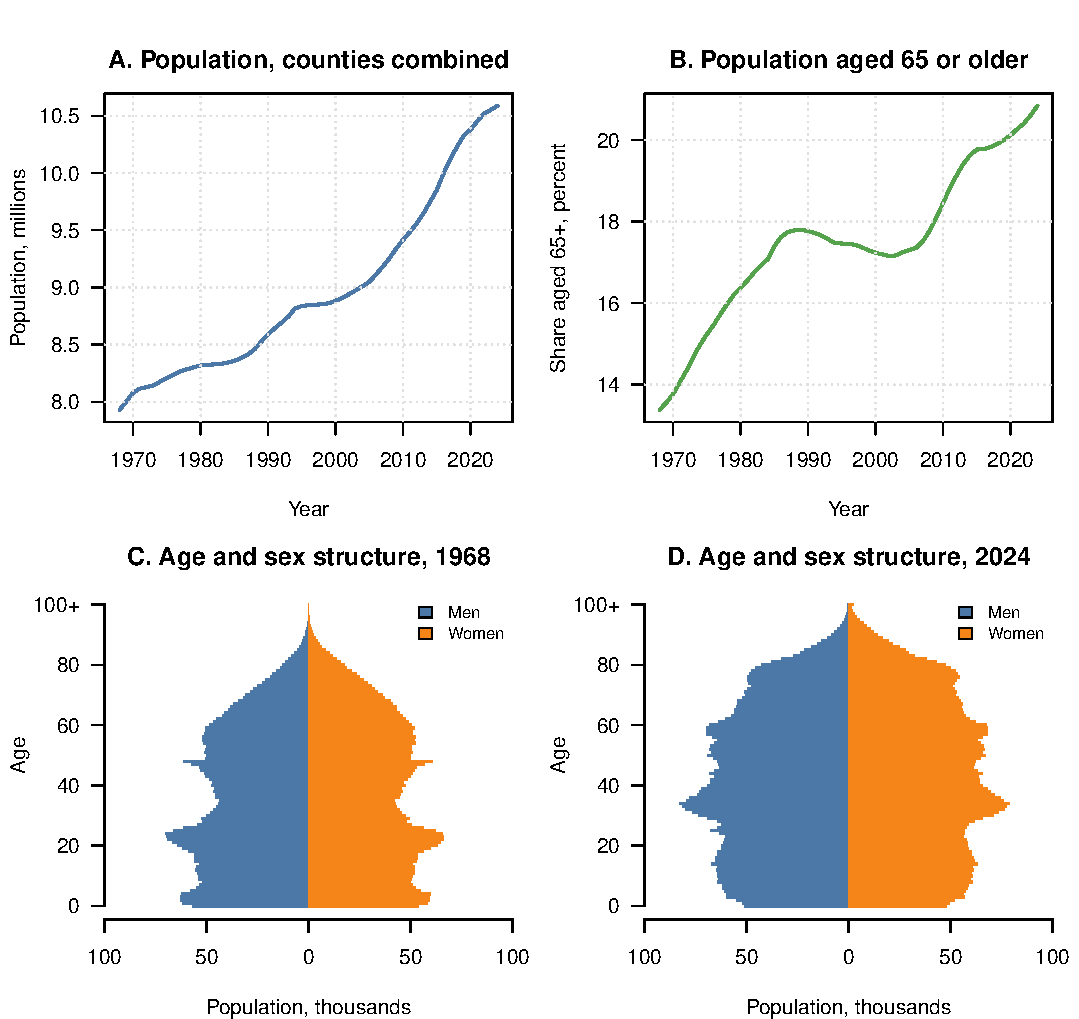
\includegraphics[width=\textwidth]{figs/case-study-population}
\caption{\label{fig:case-study-population}Population development in
Sweden based on Statistics Sweden table \code{TAB638}.
The data are downloaded at county level for all years from 1968 to 2024, all
single-year age groups from 0 to 100+, both sexes, and all
marital-status categories.
The request contains 967,176 cells and is split by \CRANpkg{pxweb} into seven API calls before being combined for analysis.}
\end{figure}
Figure~\ref{fig:case-study-population} shows that the population grew from 7.93 million in 1968 to 10.59 million in 2024.
Over the same period, the share aged 65 or older rose from 13.4\% to 20.8\%, calculated by dividing the sum of counts at ages 65 and older by the total for each year.
The two population pyramids use the same horizontal scale to compare age and sex structure across the two years.

\section{Discussion}
\label{sec:discussion}

The \CRANpkg{pxweb} package provides access to official statistics shared through PxWeb APIs.
It supports the full workflow from API discovery and metadata inspection to query construction, retrieval, conversion, comments, codelists, and citation.
In doing so, it helps users move from interactive table browsing to scripted, transparent, and reproducible statistical workflows following the tidy data principles \citep{tidyverse2019, Wickham2014tidy}.

The package has matured through active development since its first CRAN release in 2014 and now includes support for PxWeb API version 2.
As an indication of use at the time of writing, CRAN download logs report 116,164 downloads between January 2014 and June 2026 \citep{CranlogsPxweb2026}.
The \href{https://CRAN.R-project.org/package=pxweb}{CRAN package index} lists \CRANpkg{BFS} \citep{BFS} and \CRANpkg{PxWebApiData} \citep{PxWebApiData} as packages that import \CRANpkg{pxweb}.
For example, the \code{PxData()} function in \CRANpkg{PxWebApiData} uses \CRANpkg{pxweb} to retrieve data, including queries that require multiple downloads.
The \CRANpkg{pixieweb} package \citep{pixieweb} lists \CRANpkg{pxweb} in its \code{Suggests} field.
The package has also been cited in research using official-statistics data, for instance in work on electronic gambling machines and socioeconomic status \citep{raisamo2019density}, income-inequality data construction \citep{Solt2019}, trends in youth violence and mortality \citep{Tanskanen2026, Hakkarainen2026}, radiation-dose modeling after the Chernobyl nuclear power plant accident \citep{Tondel2025}, and programmatic access to open statistical data for population studies \citep{willekens2023sdmx}.

However, PxWeb installations differ across providers, with different provider-side query limits and rate limits, and APIs can change independently of the \CRANpkg{pxweb} package.
These issues motivate the package's emphasis on provider config handling, metadata validation, and request splitting.

More broadly, \CRANpkg{pxweb} contributes to the open data science ecosystem \citep{lahti2018open} by making official statistics easier to retrieve, document, and reuse in R.
The package does not replace provider documentation, but it gives researchers, public-sector analysts, educators, and civic users a common programmatic interface to a widely used dissemination infrastructure.

\clearpage

\section{Appendix: Bundled API catalogue}


\begin{table}[!htbp]
\centering
\scriptsize
\begin{tabular}{@{}>{\raggedright\arraybackslash}p{0.30\textwidth}>{\raggedright\arraybackslash}p{0.46\textwidth}>{\raggedright\arraybackslash}p{0.14\textwidth}@{}}
\toprule
Entry & Provider & Language\\
\midrule
\url{web.dzs.hr} & Croatian Bureau of Statistics & en\\
\url{andmed.stat.ee} & Estonia -- official statistics & en, et\\
\url{statistika.tai.ee} & Estonian Health Statistics and Health Research Database & en\\
\url{tilastot.etk.fi} & Finnish Centre for Pensions & en\\
\url{tilastot.tela.fi} & Finnish Pension Alliance statistics & en\\
\url{trafi2.stat.fi} & Finnish Transport Safety Agency & en, sv, fi\\
\url{px.web.ined.fr} & Generations and Gender Contextual Database & en\\
\url{pc-axis.geostat.ge} & Geostat Statistics Database & en\\
\url{stat.hel.fi} & Helsingin seudun aluesarjat -tilastotietokanta & fi\\
\url{pxweb.irena.org} & International Renewable Energy Agency & en\\
\url{www6.poderjudicial.es} & Judicial statistics, Spain & es\\
\url{data.stat.gov.lv} & Latvia -- official statistics & en, lv\\
\url{statistika.spkc.gov.lv} & Latvian Health Statistics Database & en\\
\url{statistik.linkoping.se} & Linkoping municipality in Sweden & sv\\
\url{statdb.luke.fi} & LUKE Natural Resources Institute Finland & en, fi, sv\\
\url{pxweb.nhwstat.org} & Nordic Health and Welfare Statistics & en\\
\url{pxweb.nordicstatistics.org} & Nordic Statistics Database & en\\
\url{openstat.psa.gov.ph} & Philippine Statistics Authority OpenSTAT & en\\
\url{www.grande-region.lu} & Portail statistique de la Grande Region & fr, de\\
\url{pxweb.stat.si} & SiStat Database & sl\\
\url{bank.stat.gl} & Statbank Greenland & en, kl, da\\
\url{makstat.stat.gov.mk} & State Statistical Office of the Republic of Macedonia & en, mk\\
\url{pxweb.asub.ax} & Statistics Aland & en, sv\\
\url{statbank.hagstova.fo} & Statistics Faroe Islands & en, fo\\
\url{statfin.stat.fi} & Statistics Finland & en, fi, sv\\
\url{px.hagstofa.is} & Statistics Iceland & en, is\\
\url{askdata.rks-gov.net} & Statistics Kosovo & en\\
\url{etab.llv.li} & Statistics Liechtenstein & en\\
\url{statbank.statistica.md} & Statistics Moldova & en, ro\\
\url{api.scb.se} & Statistics Sweden & en, sv\\
\url{www.pxweb.bfs.admin.ch} & Statistics Switzerland & en, de, fr\\
\url{m02-http-pxwebb.login.sundsvall.se} & Sundsvall municipality in Sweden & sv\\
\url{statistik.tillvaxtanalys.se} & Swedish Agency for Growth Policy Analysis & sv\\
\url{statistik.csn.se} & Swedish Board of Student Finance & sv\\
\url{pxexternal.energimyndigheten.se} & Swedish Energy Agency & en\\
\url{skogsstatistik.slu.se} & Swedish University of Agricultural Sciences forest statistics & en\\
\url{fohm-app.folkhalsomyndigheten.se} & The Public Health Agency of Sweden & sv\\
\url{statistik.sjv.se} & The Swedish Agricultural Agency & sv\\
\url{pxweb.skogsstyrelsen.se} & The Swedish Forest Agency & en\\
\url{statistik.konj.se} & The Swedish National Institute of Economic Research & en, sv\\
\url{prognos.konj.se} & Swedish National Institute of Economic Research, forecast database & sv\\
\url{w3.unece.org} & United Nations Economic Commission for Europe & en\\
\url{statistik.vasteras.se} & Vasteras municipality in Sweden & sv\\
\url{pxweb2022.vgregion.se} & Vastra Gotaland Region in Sweden & sv\\
\url{vero2.stat.fi} & Verohallinto -- Finnish Tax Administration & en, fi, sv\\
\url{visitfinland.stat.fi} & Visit Finland (Rudolf service) & fi\\
\bottomrule
\end{tabular}
\caption{\label{tab:api-catalogue}Bundled PxWeb API catalogue entries in \CRANpkg{pxweb}. The table lists the catalogue key, provider description, and available languages.}
\end{table}

\section{Acknowledgments}

We are grateful to all package contributors and Pyry Kantanen and Jeba
Akewak for technical assistance. The work has been supported by the
Research Council of Finland (decision 372345 to LL), and is part of
\href{https://ropengov.org/}{rOpenGov}.

\bibliography{paperRJ}

\address{M\r{a}ns Magnusson\\
  Department of Statistics\\
  Uppsala University\\
  Sweden\\
  \email{mons.magnusson@gmail.com}}

\address{Leo Lahti\\
  Department of Computing\\
  University of Turku\\
  Finland\\
  \email{leo.lahti@iki.fi}}
